\documentclass[11pt]{article}

\usepackage[a4paper,margin=1in]{geometry}
\usepackage{iftex}
\ifPDFTeX
  \usepackage[T1]{fontenc}
  \usepackage[utf8]{inputenc}
\else
  \usepackage{fontspec}
  \IfFileExists{xeCJK.sty}{\usepackage{xeCJK}}{}
\fi
\usepackage{amsmath}
\usepackage{booktabs}
\usepackage{graphicx}
\usepackage{float}
\usepackage{placeins}
\usepackage{hyperref}
\usepackage[numbers]{natbib}
\usepackage{longtable}
\usepackage{array}
\usepackage{pdflscape}

\title{MFE5210 Final Assignment: A-Share Alpha Factor Research, Signal Fusion, and Out-of-Sample Portfolio Construction}
\author{Guo Xiaoyou}
\date{April 25, 2026}

\begin{document}
\maketitle

\begin{abstract}
This report studies whether a library of daily A-share alpha factors can be combined into a stable out-of-sample stock-selection strategy under a strictly time-ordered research process. Two evaluation routes are reported: a fixed training/testing split and an annual rolling walk-forward design. All strategy-level performance metrics in the final report are stated net of one-way transaction costs of 3.6 basis points, while the single-factor diagnostic table remains gross of cost. The best fixed-split result and the best rolling result are both reported in the main text so that the reader can compare a single holdout design with a continuously updated research design.
\end{abstract}

\section{Research Objective}

The purpose of this project is to build a complete and auditable multi-factor research pipeline for A-share stock selection. The goal is not simply to report a high historical backtest; the goal is to show how factor ideas are transformed into a trading strategy through a sequence that can be defended academically: data construction, factor definition, single-factor diagnosis, factor screening, factor fusion, portfolio formation, and final out-of-sample evaluation.

The central question raised in this assignment is whether the research procedure contains look-ahead bias. That concern is valid. If one first tests all single factors on the full 2012--2026 sample and then uses the best full-sample factors to build a multi-factor model that is again evaluated on the same 2012--2026 period, the resulting strategy is not a genuine forecast test. It is an in-sample construction, because future outcomes have already influenced which factors were allowed to enter the model. For this reason, the final report does not use a full-sample ``pick-the-winners and retest'' design as the main evidence.

Instead, the report adopts two out-of-sample protocols. The fixed route asks whether factors selected before 2022 remain effective after 2022. The rolling route asks whether the same research rules continue to work when the factor set and factor weights are re-estimated each year using only the recent past. Reporting both routes is useful because they answer different questions. The fixed route is the cleaner final holdout test, while the rolling route is closer to how a live research desk would update a strategy through time.

\section{Research Design and No-Look-Ahead Protocol}

\subsection{What is learned in the training window}

The current strategy does \emph{not} use a separate validation period. This is an intentional design choice. The factor-screening rules, the portfolio construction rule, the long-short bucket size, the exit buffer, and the candidate weighting formulas are all specified ex ante. Inside each training window, the model estimates only the objects that should legitimately be learned from past data:

\begin{enumerate}
    \item the trading direction of each factor, namely whether a factor should be used as-is or reversed;
    \item the training-window quality statistics of each factor, such as long-short Sharpe, IC, Rank IC, ICIR, Rank-ICIR, win rate, and drawdown;
    \item the final admitted factor set after quality, correlation, and incremental-contribution filters;
    \item the factor weights used to build the composite stock score.
\end{enumerate}

Once these objects are estimated, the subsequent test window is used only for final evaluation. Daily scores are recomputed from same-day factor exposures, but the factor set and factor weights themselves are not allowed to depend on future test-period returns.

\subsection{Fixed train-test route}

The fixed route divides the sample into one long training interval and one final holdout interval.

\begin{itemize}
    \item Training period: January 4, 2012 to December 31, 2021.
    \item Test period: January 4, 2022 to April 20, 2026.
\end{itemize}

Everything that determines the strategy structure is learned only from the training period. The test period is then used once, without refitting, to evaluate the resulting model. This route is the more conservative design because it asks whether a model chosen entirely before 2022 still works in later market conditions.

\subsection{Rolling walk-forward route}

The rolling route uses a five-year training window and a one-year trading window.

\begin{itemize}
    \item Each trading year \(Y\) is trained on the five complete calendar years \(Y-5\) to \(Y-1\).
    \item The selected factor set and factor weights are estimated at the beginning of year \(Y\).
    \item Those decisions are then held fixed throughout year \(Y\).
\end{itemize}

For example, the 2017 trading window is trained on 2012--2016, the 2018 trading window is trained on 2013--2017, and so on. The first out-of-sample trading date is January 3, 2017. The final window covers January 1, 2026 to April 20, 2026. This route avoids look-ahead bias because every annual decision is estimated only from information that existed before the corresponding trading year.

\section{Data, Panel Construction, and Candidate Library}

The research universe is the union of the CSI 300 (HS300, 沪深300) and CSI 500 (ZZ500, 中证500) stocks used in the project panel. The final research panel spans from January 4, 2012 to April 20, 2026. It contains the securities that appear in that research universe during the sample, together with daily membership indicators and industry labels used in the neutralization step. The processed panel summary is reported in Table~\ref{tab:panel_summary}.

\begin{table}[H]
\centering
\caption{Processed research panel summary}
\label{tab:panel_summary}
\begin{tabular}{lr}
\toprule
Metric & Value \\
\midrule
Sample start & 2012-01-04 \\
Sample end & 2026-04-20 \\
Trading dates & 3469 \\
Stock-day observations & 2699059 \\
Unique securities & 1752 \\
Industry coverage & 93.66\\% \\
\bottomrule
\end{tabular}

\end{table}

Table~\ref{tab:industry_coverage} reports the industry-label coverage used by the neutralization module. The Baostock industry file used in this project is a static snapshot rather than a point-in-time historical industry panel. It contains 5,518 stock records, of which 5,199 have non-empty CSRC industry labels, spanning 83 distinct CSRC industry categories. The coverage is not perfect, but it is sufficiently broad for cross-sectional industry control and is explicitly disclosed so that the remaining limitation is visible to the reader.

\begin{table}[H]
\centering
\caption{Industry coverage in the research panel}
\label{tab:industry_coverage}
\begin{tabular}{lr}
\toprule
Metric & Value \\
\midrule
Unique panel securities & 1752 \\
Securities with industry label & 1641 \\
Industry coverage & 93.66\% \\
Baostock industry rows & 5518 \\
Distinct industry names & 83 \\
\bottomrule
\end{tabular}

\end{table}

The candidate library contains 60 reproducible daily factors built from publicly available price, volume, turnover, valuation, and WorldQuant-style price-volume formulas. The factor families include momentum, reversal, gap drift, rolling traded amount, rolling turnover, valuation level/z-score, range-volatility, and WorldQuant-style formulaic alphas. The source literature recorded in the original factor workbook includes public Chinese broker reports on price-volume factors, turnover factors, volatility factors, generalized reversal factors, and WorldQuant-style alpha formulas \citep{worldquant_101_alphas,haitong_two_sided_volatility_2017,gtja_short_cycle_price_volume_2017,pacific_generalized_reversal_2024,northeast_fund_leverage_2024,huatai_momentum_2016,huatai_turnover_2017,huatai_volatility_2017}. The exact operator definitions and factor formulas are reported in the appendices rather than repeated inline.

The basic return variable used throughout the report is the next-day forward return:
\[
fwd\_ret\_{1d,i,t} = \frac{close_{i,t+1}}{close_{i,t}} - 1.
\]
All daily strategy returns are computed by applying positions formed at date \(t\) to \(fwd\_ret\_{1d,i,t}\). This timing convention is important because it ensures that the score at date \(t\) is paired with the return realized after the score is observed.

\section{Single-Factor Testing, Sign Alignment, and Reported Metrics}

\subsection{Why factor direction must be estimated}

Not every economically useful factor is positively related to next-day return in raw form. Some factors are naturally contrarian. For example, a higher short-term reversal exposure may predict a \emph{lower} next-day return, which means the profitable trading rule is to rank the factor in reverse. Reporting such a factor with a negative Sharpe ratio and then silently reversing it later would be confusing. Therefore the final report uses \emph{aligned} single-factor metrics.

For each factor \(k\), the training window first computes the raw average Rank IC and the raw annualized long-short return. The direction rule is
\[
s_k=
\begin{cases}
+1, & \text{if the training-window Rank IC and long-short annualized return are both positive,}\\
-1, & \text{if the training-window Rank IC and long-short annualized return are both negative,}\\
\text{drop}, & \text{otherwise.}
\end{cases}
\]
If \(s_k=-1\), the factor is used in reverse. If the sign is unstable, meaning the Rank IC and the long-short spread disagree, the factor is dropped from the candidate set for that training window.

\subsection{How aligned metrics are computed}

After determining \(s_k\), the aligned factor return series and aligned factor long-short series are
\[
\text{AlignedFactorReturn}_{k,t}=s_k \cdot \text{FactorReturn}_{k,t},
\qquad
\text{AlignedLS}_{k,t}=s_k \cdot \text{RawLS}_{k,t}.
\]
All training-window Sharpe ratios, IC statistics, win rates, drawdowns, and selection filters are then computed on the aligned series. In other words, if a factor is useful only after reversal, the report presents the reversed factor as the economically meaningful version. This is the reason the appendix does not leave profitable reversed factors with negative Sharpe ratios.

\subsection{Single-factor diagnostic statistics}

The training-window single-factor diagnostics include:

\begin{itemize}
    \item factor annualized return and factor Sharpe ratio, based on the cross-sectional factor-return series;
    \item annualized long-short return and long-short Sharpe ratio, based on top-minus-bottom factor portfolios;
    \item mean IC and mean Rank IC;
    \item ICIR and Rank-ICIR;
    \item monthly win rate of the aligned long-short series;
    \item recent aligned long-short Sharpe, computed from the last 252 trading days of the training window;
    \item maximum drawdown of the aligned long-short series.
\end{itemize}

The appendix reports the full aligned single-factor table, including the final sign, the selection stage, and the incremental contribution of each candidate. This appendix is intended to make the screening process fully traceable instead of leaving factor admission as a black box.

\section{Production-Grade Factor Selection}

In this report, ``production-grade factor selection'' means a train-window-only screening process that does not rely on one summary number alone. The objective is not merely to find a factor that was strong in isolation, but to find a set of factors that is directionally stable, statistically strong, sufficiently diversified, and incrementally useful when combined.

\subsection{Step 1: summarize every factor in the training window}

For each training window, every candidate factor receives the aligned diagnostics described above. These diagnostics are computed only from the training data available before the test window begins.

\subsection{Step 2: build a robust score}

The robust score is used only for ranking candidates during screening. It is not the trading return itself. For factor \(k\),
\[
\text{RobustScore}_k
=
\frac{
Z(\text{LSSharpe}_k)
+ Z(\text{RankICIR}_k)
+ Z(\text{ICIR}_k)
+ Z(\text{MonthlyWinRate}_k)
+ Z(\text{RecentLSSharpe}_k)
}{5}
- |\text{MaxDrawdown}_k|.
\]
Each \(Z(\cdot)\) term is a cross-factor z-score computed inside the current training window. The first five terms reward profitability and stability. The final term penalizes factors that achieved good summary statistics only by accepting severe drawdowns.

\subsection{Step 3: apply hard quality filters}

After ranking candidates by robust score, the model enforces minimum quality thresholds:

\begin{itemize}
    \item aligned long-short Sharpe ratio must be at least 0.8;
    \item aligned Rank-ICIR must be at least 1.0;
    \item factors with unstable sign are discarded immediately.
\end{itemize}

These thresholds remove factors that look attractive by one statistic but remain too weak or too noisy overall.

\subsection{Step 4: apply the correlation filter}

Suppose a set of factors has already been selected. A new candidate can be admitted only if its absolute correlation with \emph{every} selected factor is no larger than 0.5. The correlation matrix is built from training-window daily factor long-short return series rather than from raw factor formulas. This design is intentional: what matters for diversification is whether two factors generate similar \emph{return behavior}, not merely whether their raw formulas look different on paper.

\subsection{Step 5: require incremental contribution}

Even if a candidate passes the quality and correlation filters, it is rejected if it does not improve the training-window composite Sharpe ratio by enough. Let \(S\) be the currently selected set and let \(k\) be the candidate. The model forms an equal-weight composite long-short return for \(S\) and for \(S \cup \{k\}\). The incremental contribution is
\[
\Delta \text{Sharpe}_k
=
\text{Sharpe}\!\left(\text{CompositeLS}(S \cup \{k\})\right)
-
\text{Sharpe}\!\left(\text{CompositeLS}(S)\right).
\]
If \(S\) is non-empty, the candidate is kept only when \(\Delta \text{Sharpe}_k \ge 0.03\). This prevents the factor list from growing merely because a factor is individually decent. A factor must also help the \emph{combined} model.

\subsection{Step 6: stop when no additional useful factor remains}

The code imposes a safety cap of 12 factors, but the effective number of factors is not fixed in advance. Factors enter only when they survive the sign check, the quality filters, the correlation filter, and the incremental-contribution filter. In the best fixed route, only four factors survive this full pipeline. In the rolling route, the number and identity of selected factors vary from year to year, which is exactly what one would expect if different market regimes favor different signal mixes.

\section{Stock Composite Score and Factor Fusion Weights}

\subsection{Composite score formula}

Once a factor set has been selected, the model assigns every stock a daily composite score:
\[
\text{Score}_{i,t}
=
\sum_{k \in S_{\tau(t)}} w_{k,\tau(t)} \tilde{x}_{i,k,t}.
\]
Each symbol in this equation has a specific meaning:

\begin{itemize}
    \item \(i\) denotes the stock.
    \item \(t\) denotes the trading date.
    \item \(\tau(t)\) denotes the training window linked to date \(t\). In the fixed route, \(\tau(t)\) is the single 2012--2021 training window for all test dates. In the rolling route, \(\tau(t)\) is the most recent five-year training window associated with the current trading year.
    \item \(S_{\tau(t)}\) is the final selected factor set estimated from that training window.
    \item \(\tilde{x}_{i,k,t}\) is the processed exposure of stock \(i\) to factor \(k\) on date \(t\). ``Processed'' means that the factor has already been sign-aligned, winsorized, z-scored, and, in the main models, neutralized.
    \item \(w_{k,\tau(t)}\) is the factor weight estimated from the training-window diagnostics.
\end{itemize}

The economic interpretation is straightforward. A stock receives a high score if it simultaneously looks attractive on multiple selected factors, especially on factors that were stronger in the training window and therefore receive larger weights.

\subsection{How factor weights are assigned}

The report compares six weight schemes:

\begin{itemize}
    \item \textbf{Equal weight:} every selected factor receives the same weight.
    \item \textbf{LS-Sharpe weight:} weights are proportional to aligned training-window long-short Sharpe.
    \item \textbf{Rank-ICIR weight:} weights are proportional to aligned training-window Rank-ICIR.
    \item \textbf{IC-mean weight:} weights are proportional to aligned training-window mean IC.
    \item \textbf{Robust-score weight:} weights are proportional to the robust score defined above.
    \item \textbf{Max-IR weight:} weights are proportional to \(\Sigma^{-1}\mu\), where \(\mu\) is the vector of aligned training-window factor long-short mean returns and \(\Sigma\) is their covariance matrix.
\end{itemize}

All reported weight schemes are constrained to be nonnegative, normalized to sum to one, and capped at 50\% per factor. The nonnegativity rule is deliberate. Because factors have already been sign-aligned, a negative combination weight would be economically hard to interpret and would effectively reintroduce reversal at the fusion stage. The 50\% cap prevents the composite from collapsing onto one factor only.

\subsection{Best fixed-route factor weights}

The best fixed-route model is the Rank-ICIR-weighted neutral long-short specification. Its selected factors and final training-window weights are reported in Table~\ref{tab:fixed_weights}.

\begin{table}[H]
\centering
\caption{Selected factors and weights for the best fixed-route model}
\label{tab:fixed_weights}
\begin{tabular}{lrrrr}
\toprule
Factor & Weight & LS Sharpe & RankICIR & Robust Score \\
\midrule
wq\_alpha\_004 & 0.313 & 1.443 & 5.739 & 1.625 \\
wq\_alpha\_002 & 0.263 & 1.246 & 4.829 & 1.173 \\
amount\_mean\_5d & 0.197 & 1.797 & 3.621 & 1.078 \\
wq\_alpha\_005 & 0.227 & 1.357 & 4.174 & 0.734 \\
\bottomrule
\end{tabular}

\end{table}

These four factors are not simply the top four single factors by one metric. They are the factors that survive the entire screening sequence and then receive weights according to their aligned Rank-ICIR in the 2012--2021 training period.

\section{Exposure Preparation and Neutralization}

Before the composite score is computed, each selected factor exposure passes through a fixed preprocessing chain:

\begin{enumerate}
    \item multiply the raw factor by the training-window sign \(s_k\);
    \item winsorize the factor cross-section by date;
    \item z-score the winsorized factor cross-section by date;
    \item if neutralization is enabled, regress the standardized exposure on style controls and industry dummies, then keep the residual.
\end{enumerate}

The main reported models use neutralization. For factor \(k\) on date \(t\), the cross-sectional regression is
\[
z_{i,k,t}
=
\alpha_{k,t}
+ \beta_{1,k,t}\log(1+\text{ADV20}_{i,t})
+ \beta_{2,k,t}\text{TurnoverProxy}_{i,t}
+ \beta_{3,k,t}\text{HS300}_{i,t}
+ \beta_{4,k,t}\text{ZZ500}_{i,t}
+ \sum_g \gamma_{g,k,t}\text{Industry}_{i,g}
+ \varepsilon_{i,k,t}.
\]
The residual \(\varepsilon_{i,k,t}\) is the neutralized exposure used in the score. Each term has a concrete interpretation:

\begin{itemize}
    \item \(\log(1+\text{ADV20})\) controls for trading-size and liquidity effects;
    \item \(\text{TurnoverProxy}\) controls short-horizon trading-activity effects;
    \item \(\text{HS300}\) and \(\text{ZZ500}\) capture broad index-membership effects;
    \item \(\text{Industry}_{i,g}\) removes average industry-level return and valuation patterns.
\end{itemize}

This step matters because two factors can appear different while still loading on the same broad industry or liquidity theme. Neutralization forces the strategy to compete on stock-specific cross-sectional information rather than simply inheriting market-structure tilts.

\section{Portfolio Construction, PnL, and Performance Metrics}

The final reported strategies are long-short portfolios. On each date \(t\), stocks are ranked by the composite score. The top 20\% enter the long side and the bottom 20\% enter the short side. Within each side, positions are equally weighted. The gross long side is normalized to \(+1\) and the gross short side is normalized to \(-1\). Therefore the daily portfolio return is
\[
r_{p,t+1}=\sum_i h_{i,t}\,fwd\_ret\_{1d,i,t},
\]
where \(h_{i,t}\) is the portfolio weight decided at date \(t\).

The strategy also uses a 25\% exit buffer. A stock already held on the long side is not immediately removed unless it falls below the top 25\% of the ranked universe; similarly, an existing short is retained unless it rises above the bottom 25\%. This rule reduces unnecessary turnover near the ranking cutoff.

The cumulative net asset value is
\[
\text{NAV}_T=\prod_{t=1}^{T}(1+r_{p,t}).
\]
The drawdown series is
\[
\text{Drawdown}_T
=
\frac{\text{NAV}_T}{\max_{s \le T}\text{NAV}_s}-1.
\]
Average one-way turnover is computed from daily position changes:
\[
\text{Turnover}_t=\frac{1}{2}\sum_i |h_{i,t}-h_{i,t-1}|.
\]
The single-factor diagnostic statistics reported in the appendix are gross of transaction costs, because they are used only to assess signal quality. By contrast, all strategy-level returns, Sharpe ratios, drawdowns, and cumulative net asset values reported in the main text are net of one-way commission costs of 3.6 basis points. Slippage is set to zero in the baseline specification because the backtest assumes close-to-close execution and does not introduce a separate intraday impact model.

The relationship between annualized performance and final NAV is also worth clarifying. CAGR is a yearly growth rate, while final NAV is the cumulative compounded result over the entire out-of-sample horizon. If the horizon length is \(Y\) years, then approximately
\[
\text{Final NAV}\approx (1+\text{CAGR})^Y.
\]
This is why a moderate annualized return can still accumulate to a much larger final NAV when the evaluation horizon is long enough.

\section{Out-of-Sample Results}

\subsection{Best model under each protocol}

Table~\ref{tab:oos_best_summary} reports the best model under each protocol.

\begin{table}[H]
\centering
\caption{Best out-of-sample model under each evaluation protocol}
\label{tab:oos_best_summary}
\resizebox{\textwidth}{!}{\begin{tabular}{llrrrr}
\toprule
Protocol & Best Model & CAGR & Sharpe & Max DD & Final NAV \\
\midrule
Fixed train-test & fixed\_rank\_icir\_ls20\_neutral\_ols & 13.71\% & 1.520 & -14.56\% & 1.73 \\
Rolling walk-forward & rolling\_robust\_score\_ls20\_neutral\_ols & 19.54\% & 2.186 & -9.85\% & 5.24 \\
\bottomrule
\end{tabular}
}
\end{table}

The fixed route and the rolling route answer different questions, so neither one replaces the other. The fixed route is the clean final holdout test. The rolling route is the more realistic ongoing research simulation. Reporting both results is therefore more informative than reporting only one backtest.

\subsection{Fixed train-test results}

Table~\ref{tab:oos_fixed} compares all fixed-route candidate fusion methods. The best specification is \texttt{fixed\_rank\_icir\_ls20\_neutral\_ols}. Its annualized return is 13.24\%, its CAGR is 13.71\%, its Sharpe ratio is 1.520, and its maximum drawdown is -14.56\%. The raw equal-weight baseline is materially worse, with a Sharpe ratio of only 0.912 and a maximum drawdown of -30.72\%.

\begin{table}[H]
\centering
\caption{Fixed train-test OOS comparison, 2022--2026}
\label{tab:oos_fixed}
\resizebox{\textwidth}{!}{\begin{tabular}{lrrrr}
\toprule
Model & Ann. Return & Sharpe & Max DD & Turnover \\
\midrule
fixed\_rank\_icir\_ls20\_neutral\_ols & 13.24\% & 1.520 & -14.56\% & 0.964 \\
fixed\_ic\_mean\_ls20\_neutral\_ols & 12.59\% & 1.438 & -14.47\% & 0.989 \\
fixed\_equal\_ls20\_neutral\_ols & 12.35\% & 1.415 & -14.86\% & 0.928 \\
fixed\_robust\_score\_ls20\_neutral\_ols & 12.07\% & 1.398 & -14.28\% & 0.948 \\
fixed\_max\_ir\_ls20\_neutral\_ols & 11.51\% & 1.335 & -14.34\% & 0.868 \\
fixed\_ls\_sharpe\_ls20\_neutral\_ols & 10.24\% & 1.205 & -14.14\% & 0.850 \\
fixed\_equal\_ls20\_raw & 12.87\% & 0.912 & -30.72\% & 0.950 \\
\bottomrule
\end{tabular}
}
\end{table}

\begin{figure}[H]
\centering
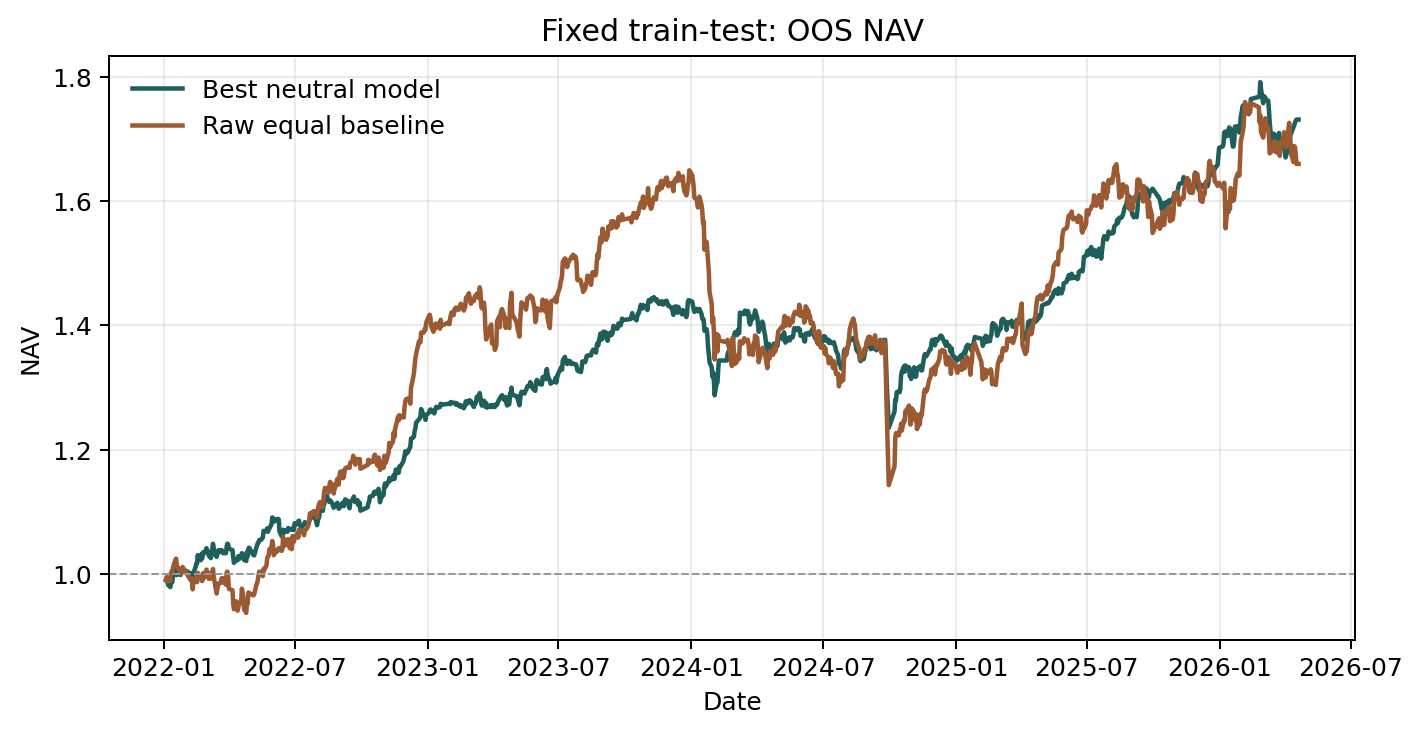
\includegraphics[width=0.88\textwidth]{assets/figures/oos_fixed_nav.png}
\caption{Fixed train-test out-of-sample NAV}
\label{fig:oos_fixed_nav}
\end{figure}

\begin{figure}[H]
\centering
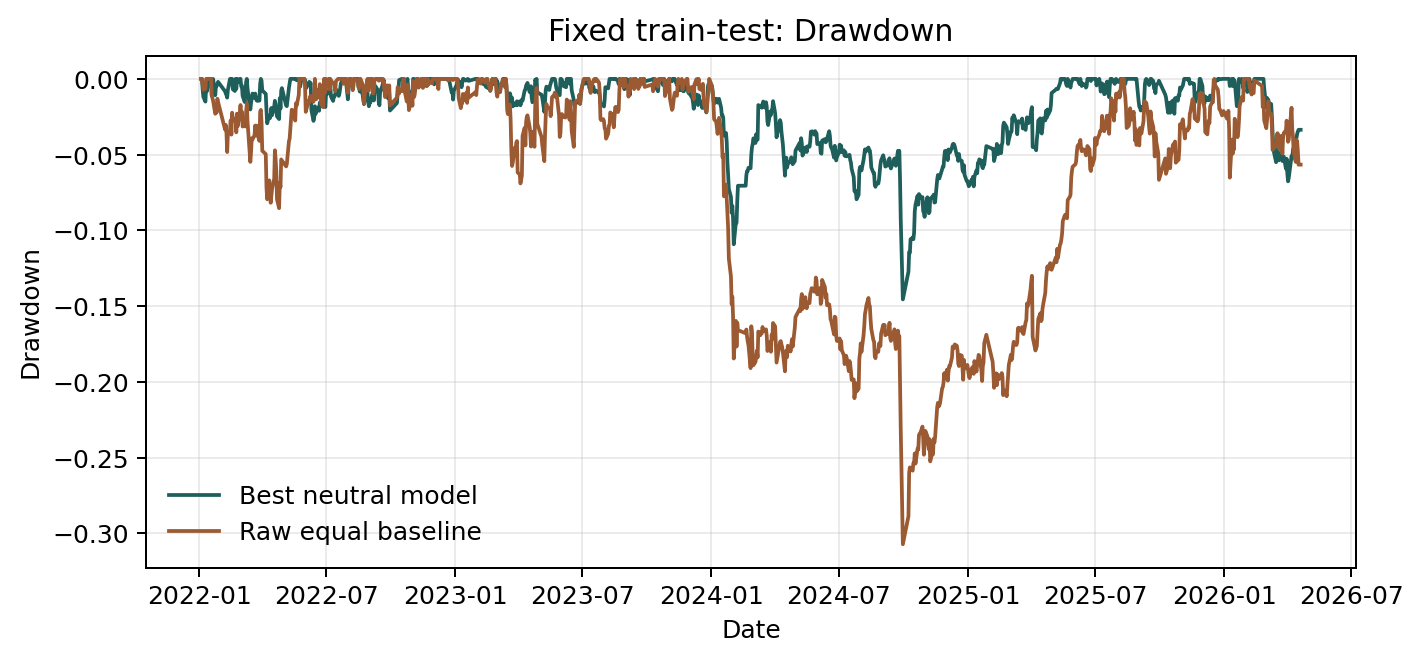
\includegraphics[width=0.88\textwidth]{assets/figures/oos_fixed_drawdown.png}
\caption{Fixed train-test out-of-sample drawdown}
\label{fig:oos_fixed_drawdown}
\end{figure}

This comparison is important because it directly answers the earlier concern that a multi-factor strategy should not become much weaker than its constituent factors without a structural reason. The raw baseline was weak because it combined unneutralized signals with no disciplined admission or weighting rule. Once the model uses aligned factors, quality filters, correlation control, incremental contribution control, and industry/style neutralization, the OOS results become much more reasonable and much more stable.

\subsection{Rolling walk-forward results}

Table~\ref{tab:oos_rolling} compares all rolling candidate fusion methods. The best specification is \texttt{rolling\_robust\_score\_ls20\_neutral\_ols}. It achieves an annualized return of 18.21\%, a CAGR of 19.54\%, a Sharpe ratio of 2.186, and a maximum drawdown of -9.85\%. The raw equal-weight baseline again performs much worse, with a Sharpe ratio of 0.841 and a maximum drawdown of -24.89\%.

\begin{table}[H]
\centering
\caption{Rolling walk-forward OOS comparison, 2017--2026}
\label{tab:oos_rolling}
\resizebox{\textwidth}{!}{\begin{tabular}{lrrrr}
\toprule
Model & Ann. Return & Sharpe & Max DD & Turnover \\
\midrule
rolling\_robust\_score\_ls20\_neutral\_ols & 18.21\% & 2.186 & -9.85\% & 1.033 \\
rolling\_rank\_icir\_ls20\_neutral\_ols & 17.95\% & 2.140 & -9.85\% & 1.037 \\
rolling\_ic\_mean\_ls20\_neutral\_ols & 17.82\% & 2.132 & -9.85\% & 1.053 \\
rolling\_equal\_ls20\_neutral\_ols & 16.60\% & 2.027 & -9.85\% & 1.020 \\
rolling\_max\_ir\_ls20\_neutral\_ols & 16.03\% & 2.019 & -9.85\% & 1.029 \\
rolling\_ls\_sharpe\_ls20\_neutral\_ols & 15.20\% & 1.872 & -9.85\% & 0.976 \\
rolling\_equal\_ls20\_raw & 11.73\% & 0.841 & -24.89\% & 0.963 \\
\bottomrule
\end{tabular}
}
\end{table}

\begin{figure}[H]
\centering
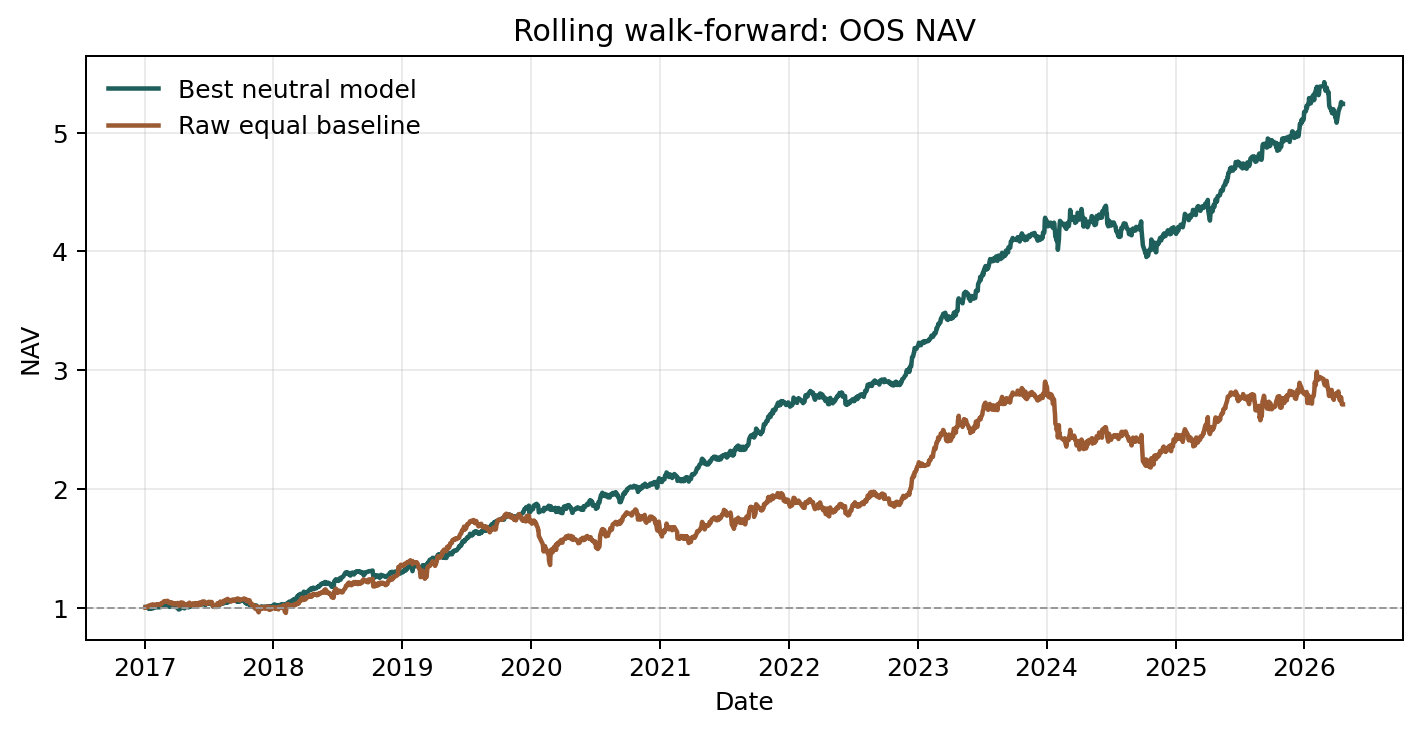
\includegraphics[width=0.88\textwidth]{assets/figures/oos_rolling_nav.png}
\caption{Rolling walk-forward out-of-sample NAV}
\label{fig:oos_rolling_nav}
\end{figure}

\begin{figure}[H]
\centering
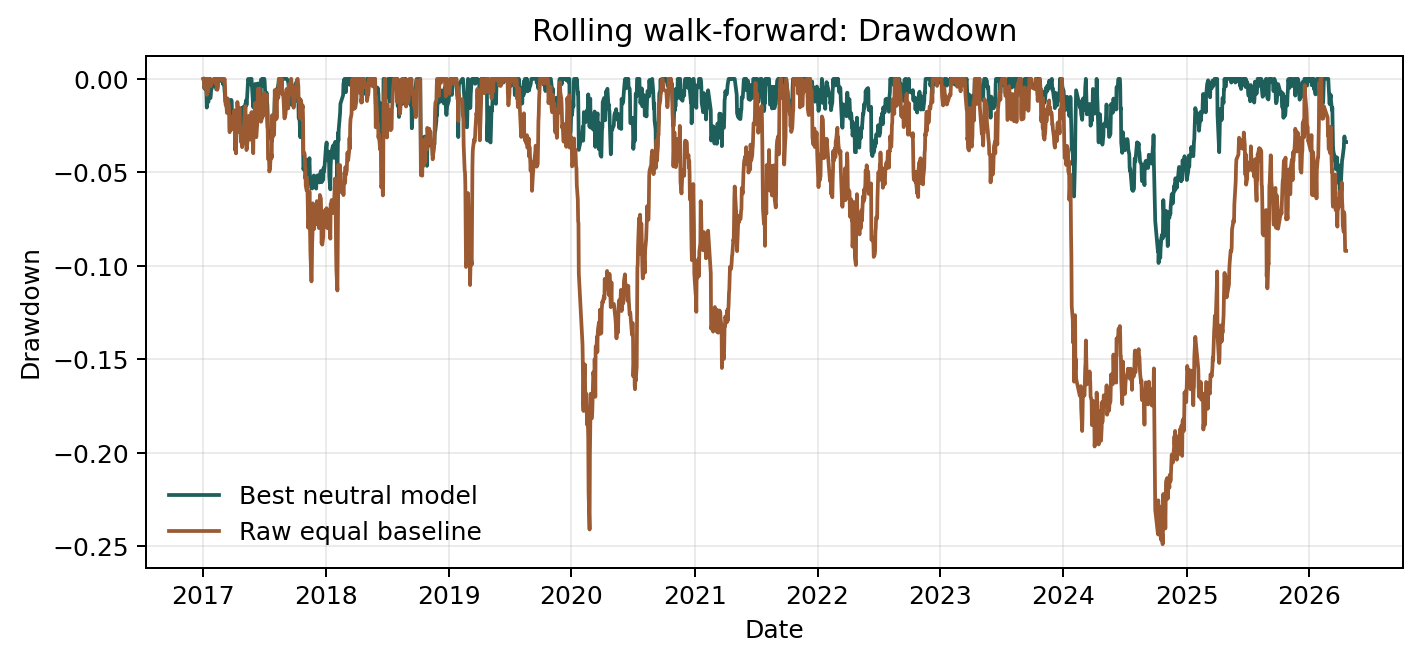
\includegraphics[width=0.88\textwidth]{assets/figures/oos_rolling_drawdown.png}
\caption{Rolling walk-forward out-of-sample drawdown}
\label{fig:oos_rolling_drawdown}
\end{figure}

The rolling models outperform the fixed models for a simple reason: the market regime changes through time, and the rolling protocol allows the factor set and factor weights to be refreshed using the most recent five years of evidence. Importantly, this is still a valid out-of-sample design, because each annual refresh is estimated only from data available before the trading year begins.

\subsection{Quantile diagnostics}

Table~\ref{tab:quantile_diag} reports annualized mean returns by score quantile for the best fixed and rolling models. The score monotonicity is not perfect in every interior bucket, but both models display a strong \(Q5-Q1\) spread, which supports the use of a long-short construction.

\begin{table}[H]
\centering
\caption{Average annualized quantile returns for the best fixed and rolling models}
\label{tab:quantile_diag}
\resizebox{\textwidth}{!}{\begin{tabular}{lrrrrrr}
\toprule
Model & Q1 & Q2 & Q3 & Q4 & Q5 & Q5-Q1 \\
\midrule
Fixed Rank-ICIR neutral & -1.25\% & 4.35\% & 7.24\% & 11.97\% & 11.87\% & 13.12\% \\
Rolling robust-score neutral & -5.35\% & 4.70\% & 9.78\% & 13.24\% & 14.79\% & 20.14\% \\
\bottomrule
\end{tabular}
}
\end{table}

The rolling robust-score model exhibits the stronger \(Q5-Q1\) spread at 20.14\%, versus 13.12\% for the fixed Rank-ICIR model. This is consistent with its higher Sharpe ratio and stronger cumulative NAV path.

\section{Discussion}

The first conclusion is methodological. A full-sample procedure that first identifies the best factors on 2012--2026 and then evaluates a multi-factor strategy on the same 2012--2026 period would indeed contain look-ahead bias. The current report avoids that bias by estimating factor direction, factor admission, and factor weights only inside the relevant training window. This makes the reported results a genuine out-of-sample evaluation rather than a full-sample reconstruction.

The second conclusion is economic. Strong single factors do not automatically produce a strong multi-factor strategy. Many price-volume factors overlap. If one simply averages them, the model can become over-concentrated in one theme, inherit unwanted industry or liquidity exposure, and turn over too aggressively around ranking cutoffs. The present design addresses those problems through sign alignment, quality thresholds, correlation control, incremental contribution control, neutralization, and explicit comparison of multiple factor-fusion schemes.

The third conclusion is comparative. The fixed route is the stricter final holdout test and therefore the more conservative performance estimate. The rolling route is the more realistic ongoing research process because it updates the factor mix annually using only newly available data. In this project, both routes are useful and both should be reported. The fixed route shows that a pre-2022 model continues to work after 2022; the rolling route shows that annual re-estimation materially improves adaptability.

\section{Limitations}

Several limitations should be kept in mind when interpreting the results.

\begin{itemize}
    \item Commission costs are deducted at 3.6 basis points one-way, but financing costs, stock-borrow constraints, price limits, and additional execution slippage are not modeled.
    \item Industry labels are used as practical controls, but they are not a complete institutional-grade point-in-time historical classification database.
    \item The research universe is limited to the CSI 300 / CSI 500 panel rather than the full A-share market.
    \item The factor library is limited to factors reproducible from the locally available data fields. Some ideas cited in the original literature workbook require proprietary data and are therefore treated as literature references rather than fully implemented production signals.
\end{itemize}

\section{Conclusion}

This report rewrites the strategy around a defensible out-of-sample research design. The current model does not select factors on the full sample and then retest them on the same sample. Instead, it uses past data to determine factor direction, select factors through a multi-step screening process, assign training-window factor weights, and then evaluate the resulting strategy on a later out-of-sample period.

Under the fixed train-test route, the best model is the Rank-ICIR-weighted neutral long-short specification, which delivers a 13.71\% CAGR, a Sharpe ratio of 1.520, and a maximum drawdown of -14.56\% over 2022--2026. Under the rolling walk-forward route, the best model is the robust-score-weighted neutral long-short specification, which delivers a 19.54\% CAGR, a Sharpe ratio of 2.186, and a maximum drawdown of -9.85\% over 2017--2026. Taken together, these results support the conclusion that the strategy becomes much more credible once the factor research process itself is placed on a no-look-ahead footing.

\appendix

\section{Operator Definitions}
\label{app:operators}
\scriptsize
\setlength{\tabcolsep}{2pt}
\begin{longtable}{p{0.20\textwidth}p{0.70\textwidth}}
\toprule
Operator & Definition \\
\midrule
\endfirsthead
\toprule
Operator & Definition \\
\midrule
\endhead
delay & delay(x,n): security-level lag of field x by n trading days. \\
mean & mean(x,n): security-level rolling arithmetic mean over n trading days. \\
std & std(x,n): security-level rolling standard deviation over n trading days. \\
diff & diff(x,n): security-level x\_t minus x\_\{t-n\}. \\
pct\_change & pct\_change(x,n): security-level x\_t / x\_\{t-n\} - 1. \\
zscore & zscore(x): cross-sectional daily z-score using same-date mean and population standard deviation. \\
winsorize & winsorize(x): cross-sectional daily clipping at the 1st and 99th percentiles. \\
rankIC & Daily Spearman rank correlation between factor exposure and next-day return. \\
IC & Daily Pearson correlation between factor exposure and next-day return. \\
residualize(x,Z) & Daily OLS residual from regressing factor x on control matrix Z. \\
\bottomrule
\end{longtable}
\normalsize


\begin{landscape}
\section{Factor Dictionary}
\label{app:factor_dict}
\scriptsize
\setlength{\tabcolsep}{2pt}
\begin{longtable}{p{0.17\textwidth}p{0.10\textwidth}p{0.10\textwidth}p{0.16\textwidth}p{0.35\textwidth}}
\toprule
Factor & Family & Aligned Sharpe & Fields & Exact formula \\
\midrule
\endfirsthead
\toprule
Factor & Family & Aligned Sharpe & Fields & Exact formula \\
\midrule
\endhead
return\_5d & momentum & 1.064 & close & close / delay(close, 5) - 1 \\
reversal\_5d & momentum & 1.064 & close & -(close / delay(close, 5) - 1) \\
gap\_drift\_5d & momentum & 0.819 & close, open & mean((close-open)/open, 5) \\
return\_10d & momentum & 0.607 & close & close / delay(close, 10) - 1 \\
reversal\_10d & momentum & 0.607 & close & -(close / delay(close, 10) - 1) \\
gap\_drift\_10d & momentum & 0.293 & close, open & mean((close-open)/open, 10) \\
return\_20d & momentum & 0.214 & close & close / delay(close, 20) - 1 \\
reversal\_20d & momentum & 0.214 & close & -(close / delay(close, 20) - 1) \\
gap\_drift\_20d & momentum & 0.225 & close, open & mean((close-open)/open, 20) \\
return\_60d & momentum & 0.109 & close & close / delay(close, 60) - 1 \\
reversal\_60d & momentum & 0.109 & close & -(close / delay(close, 60) - 1) \\
gap\_drift\_60d & momentum & -0.031 & close, open & mean((close-open)/open, 60) \\
return\_120d & momentum & 0.325 & close & close / delay(close, 120) - 1 \\
reversal\_120d & momentum & 0.325 & close & -(close / delay(close, 120) - 1) \\
gap\_drift\_120d & momentum & -0.347 & close, open & mean((close-open)/open, 120) \\
return\_240d & momentum & 0.440 & close & close / delay(close, 240) - 1 \\
reversal\_240d & momentum & 0.440 & close & -(close / delay(close, 240) - 1) \\
gap\_drift\_240d & momentum & -0.543 & close, open & mean((close-open)/open, 240) \\
volatility\_5d & volatility & 1.184 & ret\_1d & std(ret\_1d, 5) \\
range\_vol\_5d & volatility & 0.832 & high, low, close & mean((high-low)/close, 5) \\
volatility\_10d & volatility & 0.673 & ret\_1d & std(ret\_1d, 10) \\
range\_vol\_10d & volatility & 0.572 & high, low, close & mean((high-low)/close, 10) \\
volatility\_20d & volatility & 0.024 & ret\_1d & std(ret\_1d, 20) \\
range\_vol\_20d & volatility & 0.695 & high, low, close & mean((high-low)/close, 20) \\
volatility\_40d & volatility & 1.216 & ret\_1d & std(ret\_1d, 40) \\
range\_vol\_40d & volatility & 0.739 & high, low, close & mean((high-low)/close, 40) \\
volatility\_60d & volatility & 1.501 & ret\_1d & std(ret\_1d, 60) \\
range\_vol\_60d & volatility & 0.896 & high, low, close & mean((high-low)/close, 60) \\
volatility\_120d & volatility & 1.410 & ret\_1d & std(ret\_1d, 120) \\
range\_vol\_120d & volatility & 0.838 & high, low, close & mean((high-low)/close, 120) \\
amount\_mean\_5d & liquidity & 0.783 & amount & mean(amount, 5) \\
turnover\_mean\_5d & liquidity & 2.884 & turn & mean(turn, 5) \\
amount\_mean\_10d & liquidity & 0.605 & amount & mean(amount, 10) \\
turnover\_mean\_10d & liquidity & 2.857 & turn & mean(turn, 10) \\
amount\_mean\_20d & liquidity & 0.452 & amount & mean(amount, 20) \\
turnover\_mean\_20d & liquidity & 2.810 & turn & mean(turn, 20) \\
amount\_mean\_40d & liquidity & -0.257 & amount & mean(amount, 40) \\
turnover\_mean\_40d & liquidity & 2.589 & turn & mean(turn, 40) \\
amount\_mean\_60d & liquidity & -0.234 & amount & mean(amount, 60) \\
turnover\_mean\_60d & liquidity & 2.486 & turn & mean(turn, 60) \\
amount\_mean\_120d & liquidity & -0.275 & amount & mean(amount, 120) \\
turnover\_mean\_120d & liquidity & 2.174 & turn & mean(turn, 120) \\
peTTM\_level & valuation & 0.454 & peTTM & peTTM \\
peTTM\_zscore & valuation & 0.454 & peTTM & zscore(peTTM) \\
pbMRQ\_level & valuation & 0.183 & pbMRQ & pbMRQ \\
pbMRQ\_zscore & valuation & 0.183 & pbMRQ & zscore(pbMRQ) \\
psTTM\_level & valuation & 0.295 & psTTM & psTTM \\
psTTM\_zscore & valuation & 0.295 & psTTM & zscore(psTTM) \\
pcfNcfTTM\_level & valuation & 0.172 & pcfNcfTTM & pcfNcfTTM \\
pcfNcfTTM\_zscore & valuation & 0.172 & pcfNcfTTM & zscore(pcfNcfTTM) \\
wq\_alpha\_001 & wq\_like & 1.494 &  & see implementation in wq\_like.py for alpha 001 \\
wq\_alpha\_002 & wq\_like & 0.568 &  & see implementation in wq\_like.py for alpha 002 \\
wq\_alpha\_003 & wq\_like & 0.005 &  & see implementation in wq\_like.py for alpha 003 \\
wq\_alpha\_004 & wq\_like & 0.076 &  & see implementation in wq\_like.py for alpha 004 \\
wq\_alpha\_005 & wq\_like & 0.556 &  & see implementation in wq\_like.py for alpha 005 \\
wq\_alpha\_006 & wq\_like & 0.277 &  & see implementation in wq\_like.py for alpha 006 \\
wq\_alpha\_007 & wq\_like & 3.612 &  & see implementation in wq\_like.py for alpha 007 \\
wq\_alpha\_008 & wq\_like & 0.389 &  & see implementation in wq\_like.py for alpha 008 \\
wq\_alpha\_009 & wq\_like & 0.498 &  & see implementation in wq\_like.py for alpha 009 \\
wq\_alpha\_010 & wq\_like & 0.080 &  & see implementation in wq\_like.py for alpha 010 \\
\bottomrule
\end{longtable}
\normalsize

\end{landscape}

\begin{landscape}
\section{Full Single-Factor Diagnostics in the Fixed Training Window}
\label{app:single_factor}
\scriptsize
\setlength{\tabcolsep}{2pt}
\begin{longtable}{lrrrrrrrrl}
\toprule
Factor & Sharpe & LS Sharpe & IC & RankIC & ICIR & RankICIR & WinRate & Robust & Rev \\
\midrule
\endfirsthead
\toprule
Factor & Sharpe & LS Sharpe & IC & RankIC & ICIR & RankICIR & WinRate & Robust & Rev \\
\midrule
\endhead
wq\_alpha\_007 & 3.612 & 2.033 & 0.022 & -0.010 & 3.568 & -1.279 & 0.686 & 1.874 & No \\
wq\_alpha\_001 & 1.494 & 0.450 & 0.010 & -0.031 & 1.087 & -3.367 & 0.488 & 1.172 & No \\
volatility\_5d & 1.184 & 1.218 & 0.007 & -0.002 & 1.194 & -0.348 & 0.640 & 0.836 & No \\
return\_5d & 1.064 & 0.172 & 0.005 & -0.031 & 0.574 & -3.440 & 0.465 & 0.976 & No \\
volatility\_10d & 0.673 & 0.827 & 0.004 & -0.005 & 0.700 & -0.923 & 0.645 & 0.728 & No \\
return\_10d & 0.607 & 0.280 & 0.003 & -0.024 & 0.293 & -2.530 & 0.512 & 0.735 & No \\
wq\_alpha\_002 & 0.568 & 1.226 & 0.012 & 0.037 & 1.611 & 4.826 & 0.669 & 1.758 & No \\
gap\_drift\_240d & 0.543 & -0.178 & 0.005 & -0.002 & 0.759 & -0.292 & 0.512 & 0.385 & Yes \\
wq\_alpha\_009 & 0.498 & 0.599 & 0.012 & 0.033 & 1.785 & 4.482 & 0.663 & 1.517 & No \\
return\_240d & 0.440 & 0.523 & 0.006 & 0.008 & 0.733 & 0.862 & 0.553 & 0.557 & No \\
gap\_drift\_120d & 0.347 & -0.172 & 0.003 & -0.005 & 0.456 & -0.648 & 0.517 & 0.401 & Yes \\
return\_120d & 0.325 & 0.356 & 0.004 & 0.002 & 0.426 & 0.283 & 0.488 & 0.279 & No \\
return\_20d & 0.214 & 0.062 & -0.000 & -0.016 & -0.025 & -1.736 & 0.509 & 0.433 & No \\
pbMRQ\_level & 0.183 & 0.056 & 0.002 & 0.001 & 0.296 & 0.154 & 0.535 & 0.016 & No \\
pbMRQ\_zscore & 0.183 & 0.056 & 0.002 & 0.001 & 0.296 & 0.154 & 0.535 & 0.016 & No \\
pcfNcfTTM\_zscore & 0.172 & 0.239 & 0.001 & 0.004 & 0.237 & 0.500 & 0.558 & 0.128 & No \\
pcfNcfTTM\_level & 0.172 & 0.239 & 0.001 & 0.004 & 0.237 & 0.500 & 0.558 & 0.128 & No \\
return\_60d & 0.109 & 0.114 & 0.001 & -0.004 & 0.144 & -0.454 & 0.503 & 0.217 & No \\
gap\_drift\_60d & 0.031 & -0.280 & 0.001 & -0.010 & 0.129 & -1.213 & 0.506 & 0.380 & Yes \\
volatility\_20d & 0.024 & 0.057 & 0.001 & 0.004 & 0.150 & 0.362 & 0.500 & 0.082 & No \\
wq\_alpha\_003 & -0.005 & -0.895 & -0.005 & -0.020 & -0.660 & -2.330 & 0.622 & 0.845 & Yes \\
wq\_alpha\_004 & -0.076 & -0.420 & -0.004 & -0.018 & -0.557 & -2.486 & 0.558 & 0.818 & Yes \\
wq\_alpha\_010 & -0.080 & -0.244 & 0.002 & 0.032 & 0.319 & 4.415 & 0.494 & 0.991 & Yes \\
reversal\_60d & -0.109 & -0.114 & -0.001 & 0.004 & -0.144 & 0.454 & 0.503 & 0.217 & Yes \\
reversal\_20d & -0.214 & -0.062 & 0.000 & 0.016 & 0.025 & 1.736 & 0.509 & 0.433 & Yes \\
gap\_drift\_20d & -0.225 & -0.429 & -0.003 & -0.021 & -0.344 & -2.327 & 0.558 & 0.708 & Yes \\
amount\_mean\_60d & -0.234 & 0.204 & -0.001 & 0.001 & -0.150 & 0.251 & 0.483 & 0.202 & No \\
amount\_mean\_40d & -0.257 & 0.158 & -0.001 & 0.002 & -0.139 & 0.332 & 0.488 & 0.204 & No \\
amount\_mean\_120d & -0.275 & 0.336 & -0.001 & 0.001 & -0.237 & 0.120 & 0.517 & 0.240 & No \\
wq\_alpha\_006 & -0.277 & -0.489 & -0.005 & -0.014 & -0.900 & -2.298 & 0.570 & 0.921 & Yes \\
gap\_drift\_10d & -0.293 & -0.529 & -0.004 & -0.026 & -0.503 & -2.986 & 0.512 & 0.879 & Yes \\
psTTM\_level & -0.295 & -0.360 & -0.002 & 0.004 & -0.259 & 0.446 & 0.512 & 0.394 & Yes \\
psTTM\_zscore & -0.295 & -0.360 & -0.002 & 0.004 & -0.259 & 0.446 & 0.512 & 0.394 & Yes \\
reversal\_120d & -0.325 & -0.356 & -0.004 & -0.002 & -0.426 & -0.283 & 0.488 & 0.279 & Yes \\
wq\_alpha\_008 & -0.389 & -0.750 & -0.004 & -0.013 & -0.452 & -1.570 & 0.535 & 0.724 & Yes \\
reversal\_240d & -0.440 & -0.523 & -0.006 & -0.008 & -0.733 & -0.862 & 0.553 & 0.557 & Yes \\
amount\_mean\_20d & -0.452 & -0.218 & -0.002 & 0.001 & -0.347 & 0.172 & 0.529 & 0.198 & Yes \\
peTTM\_level & -0.454 & -0.429 & -0.003 & -0.004 & -0.505 & -0.478 & 0.541 & 0.440 & Yes \\
peTTM\_zscore & -0.454 & -0.429 & -0.003 & -0.004 & -0.505 & -0.478 & 0.541 & 0.440 & Yes \\
wq\_alpha\_005 & -0.556 & -0.407 & -0.004 & -0.003 & -0.550 & -0.350 & 0.517 & 0.320 & Yes \\
range\_vol\_10d & -0.572 & -0.328 & -0.003 & -0.018 & -0.382 & -2.566 & 0.523 & 0.770 & Yes \\
amount\_mean\_10d & -0.605 & -0.520 & -0.002 & -0.002 & -0.508 & -0.446 & 0.610 & 0.483 & Yes \\
reversal\_10d & -0.607 & -0.280 & -0.003 & 0.024 & -0.293 & 2.530 & 0.512 & 0.735 & Yes \\
range\_vol\_20d & -0.695 & -0.339 & -0.003 & -0.014 & -0.432 & -1.934 & 0.535 & 0.571 & Yes \\
range\_vol\_40d & -0.739 & -0.537 & -0.004 & -0.011 & -0.479 & -1.444 & 0.593 & 0.606 & Yes \\
amount\_mean\_5d & -0.783 & -0.645 & -0.004 & -0.006 & -0.756 & -1.238 & 0.593 & 0.783 & Yes \\
gap\_drift\_5d & -0.819 & -1.005 & -0.011 & -0.036 & -1.342 & -4.105 & 0.628 & 1.435 & Yes \\
range\_vol\_5d & -0.832 & -0.571 & -0.006 & -0.022 & -0.797 & -3.212 & 0.576 & 1.105 & Yes \\
range\_vol\_120d & -0.838 & -0.763 & -0.005 & -0.011 & -0.712 & -1.440 & 0.570 & 0.747 & Yes \\
range\_vol\_60d & -0.896 & -0.754 & -0.005 & -0.011 & -0.673 & -1.504 & 0.576 & 0.740 & Yes \\
reversal\_5d & -1.064 & -0.172 & -0.005 & 0.031 & -0.574 & 3.440 & 0.465 & 0.976 & Yes \\
volatility\_40d & -1.216 & -1.227 & -0.007 & -0.006 & -1.123 & -0.941 & 0.657 & 0.909 & Yes \\
volatility\_120d & -1.410 & -1.287 & -0.010 & -0.012 & -1.407 & -1.624 & 0.622 & 1.115 & Yes \\
volatility\_60d & -1.501 & -1.353 & -0.009 & -0.010 & -1.459 & -1.464 & 0.657 & 1.165 & Yes \\
turnover\_mean\_120d & -2.174 & -2.578 & -0.013 & -0.007 & -2.199 & -1.104 & 0.738 & 1.636 & Yes \\
turnover\_mean\_60d & -2.486 & -2.701 & -0.015 & -0.007 & -2.487 & -1.123 & 0.767 & 1.718 & Yes \\
turnover\_mean\_40d & -2.589 & -2.757 & -0.016 & -0.007 & -2.571 & -1.137 & 0.785 & 1.721 & Yes \\
turnover\_mean\_20d & -2.810 & -2.914 & -0.017 & -0.008 & -2.804 & -1.288 & 0.762 & 1.792 & Yes \\
turnover\_mean\_10d & -2.857 & -3.108 & -0.019 & -0.011 & -2.919 & -1.875 & 0.797 & 2.098 & Yes \\
turnover\_mean\_5d & -2.884 & -3.139 & -0.020 & -0.017 & -3.048 & -2.649 & 0.791 & 2.325 & Yes \\
\bottomrule
\end{longtable}
\normalsize

\end{landscape}

\begin{landscape}
\section{Rolling Walk-Forward Selection Details}
\label{app:selection_details}
\scriptsize
\setlength{\tabcolsep}{2pt}
\begin{longtable}{lrrrrrl}
\toprule
Factor & Cluster & Rank & Robust & Recent & MDD & Stage \\
\midrule
\endfirsthead
\toprule
Factor & Cluster & Rank & Robust & Recent & MDD & Stage \\
\midrule
\endhead
turnover\_mean\_5d & 14 & 1 & 2.325 & 0.492 & -0.182 & selected \\
turnover\_mean\_10d & 14 & 2 & 2.098 & 0.205 & -0.164 & cluster\_redundant \\
wq\_alpha\_007 & 24 & 1 & 1.874 & 0.431 & -0.239 & selected \\
turnover\_mean\_20d & 14 & 3 & 1.792 & -0.484 & -0.208 & cluster\_redundant \\
wq\_alpha\_002 & 19 & 1 & 1.758 & 0.991 & -0.598 & selected \\
turnover\_mean\_40d & 14 & 4 & 1.721 & -0.091 & -0.190 & cluster\_redundant \\
turnover\_mean\_60d & 14 & 5 & 1.718 & 0.176 & -0.172 & cluster\_redundant \\
turnover\_mean\_120d & 14 & 6 & 1.636 & 0.408 & -0.166 & cluster\_redundant \\
wq\_alpha\_009 & 26 & 1 & 1.517 & 1.130 & -0.852 & correlation\_blocked \\
gap\_drift\_5d & 4 & 1 & 1.435 & 0.071 & -0.261 & selected \\
wq\_alpha\_001 & 4 & 2 & 1.172 & 0.206 & -0.344 & cluster\_redundant \\
volatility\_60d & 17 & 1 & 1.165 & 0.399 & -0.153 & selected \\
volatility\_120d & 11 & 1 & 1.115 & 0.129 & -0.177 & correlation\_blocked \\
range\_vol\_5d & 10 & 1 & 1.105 & 0.509 & -0.364 & selected \\
wq\_alpha\_010 & 27 & 1 & 0.991 & -0.106 & -0.403 & correlation\_blocked \\
reversal\_5d & 4 & 3 & 0.976 & 0.189 & -0.356 & cluster\_redundant \\
return\_5d & 4 & 4 & 0.976 & 0.189 & -0.356 & cluster\_redundant \\
wq\_alpha\_006 & 23 & 1 & 0.921 & 0.991 & -0.334 & selected \\
volatility\_40d & 17 & 2 & 0.909 & 0.213 & -0.206 & cluster\_redundant \\
gap\_drift\_10d & 1 & 1 & 0.879 & 0.103 & -0.341 & correlation\_blocked \\
wq\_alpha\_003 & 20 & 1 & 0.845 & -0.014 & -0.218 & correlation\_blocked \\
volatility\_5d & 18 & 1 & 0.836 & 0.464 & -0.151 & correlation\_blocked \\
wq\_alpha\_004 & 21 & 1 & 0.818 & 0.669 & -0.328 & correlation\_blocked \\
amount\_mean\_5d & 0 & 1 & 0.783 & 0.818 & -0.202 & correlation\_blocked \\
range\_vol\_10d & 10 & 2 & 0.770 & 0.353 & -0.552 & cluster\_redundant \\
range\_vol\_120d & 11 & 2 & 0.747 & 0.182 & -0.348 & cluster\_redundant \\
range\_vol\_60d & 11 & 3 & 0.740 & 0.106 & -0.427 & cluster\_redundant \\
reversal\_10d & 1 & 2 & 0.735 & 0.220 & -0.403 & cluster\_redundant \\
return\_10d & 1 & 3 & 0.735 & 0.220 & -0.403 & cluster\_redundant \\
volatility\_10d & 15 & 1 & 0.728 & 0.656 & -0.236 & correlation\_blocked \\
wq\_alpha\_008 & 25 & 1 & 0.724 & 0.428 & -0.250 & selected \\
gap\_drift\_20d & 1 & 4 & 0.708 & 0.235 & -0.378 & cluster\_redundant \\
range\_vol\_40d & 11 & 4 & 0.606 & 0.033 & -0.460 & cluster\_redundant \\
range\_vol\_20d & 11 & 5 & 0.571 & -0.321 & -0.521 & cluster\_redundant \\
return\_240d & 13 & 1 & 0.557 & 0.542 & -0.483 & selected \\
reversal\_240d & 13 & 2 & 0.557 & 0.542 & -0.483 & cluster\_redundant \\
amount\_mean\_10d & 0 & 2 & 0.483 & 0.485 & -0.203 & cluster\_redundant \\
peTTM\_level & 8 & 1 & 0.440 & 0.574 & -0.343 & selected \\
peTTM\_zscore & 8 & 2 & 0.440 & 0.574 & -0.343 & cluster\_redundant \\
reversal\_20d & 1 & 5 & 0.433 & 0.300 & -0.468 & cluster\_redundant \\
return\_20d & 1 & 6 & 0.433 & 0.300 & -0.468 & cluster\_redundant \\
gap\_drift\_120d & 2 & 1 & 0.401 & 0.885 & -0.585 & correlation\_blocked \\
psTTM\_zscore & 9 & 1 & 0.394 & 0.842 & -0.389 & selected \\
psTTM\_level & 9 & 2 & 0.394 & 0.842 & -0.389 & cluster\_redundant \\
gap\_drift\_240d & 3 & 1 & 0.385 & 0.757 & -0.507 & correlation\_blocked \\
gap\_drift\_60d & 5 & 1 & 0.380 & 0.287 & -0.491 & correlation\_blocked \\
wq\_alpha\_005 & 22 & 1 & 0.320 & -0.123 & -0.346 & selected \\
reversal\_120d & 12 & 2 & 0.279 & 0.143 & -0.405 & cluster\_redundant \\
return\_120d & 12 & 1 & 0.279 & 0.143 & -0.405 & correlation\_blocked \\
amount\_mean\_120d & 0 & 3 & 0.240 & 0.295 & -0.322 & cluster\_redundant \\
return\_60d & 5 & 2 & 0.217 & 0.445 & -0.477 & cluster\_redundant \\
reversal\_60d & 5 & 3 & 0.217 & 0.445 & -0.477 & cluster\_redundant \\
amount\_mean\_40d & 0 & 4 & 0.204 & 0.264 & -0.365 & cluster\_redundant \\
amount\_mean\_60d & 0 & 5 & 0.202 & 0.262 & -0.339 & cluster\_redundant \\
amount\_mean\_20d & 0 & 6 & 0.198 & -0.058 & -0.352 & cluster\_redundant \\
pcfNcfTTM\_zscore & 7 & 1 & 0.128 & -0.634 & -0.451 & selected \\
pcfNcfTTM\_level & 7 & 2 & 0.128 & -0.634 & -0.451 & cluster\_redundant \\
volatility\_20d & 16 & 1 & 0.082 & -0.183 & -0.439 & selected \\
pbMRQ\_level & 6 & 1 & 0.016 & -0.505 & -0.616 & selected \\
pbMRQ\_zscore & 6 & 2 & 0.016 & -0.505 & -0.616 & cluster\_redundant \\
\bottomrule
\end{longtable}
\normalsize

\end{landscape}

\nocite{worldquant_101_alphas,haitong_two_sided_volatility_2017,gtja_short_cycle_price_volume_2017,pacific_generalized_reversal_2024,northeast_fund_leverage_2024,huatai_momentum_2016,huatai_turnover_2017,huatai_volatility_2017}
\bibliographystyle{plainnat}
\bibliography{references}

\end{document}
